\section{KI-Suchverfahren}

Es gibt zwei Klassen von Suchverfahren: \textbf{blinde Suchverfahren} und \textbf{KI-Suchverfahren}. Blinde Suchverfahren sind auf einem bestimmten Schema basiert, das unabh�ngig von dem jeweiligen Problem ist. Einige Beispiele hierf�r sind die in den vorangegangenen Kapiteln behandelten Verfahren wie Breitensuche, Tiefensuche, Biridketionale Suche usw. 

KI-Suchverfahren hingegen nutzen problemspezifisches Vorwissen zur Eingrenzung des Suchraums. Es handelt sich um informierte heuristische Suchverfarhen.

\textbf{Blinde Suchverfahren} erfordern, dass eine L�sung durch systematische und ersch�pfende Suche in einem Suchgraphen gefunden wird, was ineffizient und kein problemspezifisches Wissen nutzt.

\textbf{Informierte Suchprozesse} hingegen nutzen problemspezifische Eigenschaften, um die Effizienz der Knotenexpansion zu verbessern.

\subsection{Greedy Search}
\label{section:greedy-search}
Die Greedy-Suche ist eine modifizierte Breitensuche (siehe Abschnitt \ref{section:breitensuche}), bei der nur die Knoten mit den geringsten Kosten in die Warteschlange aufgenommen werden. 

\paragraph{Ablauf von Greedy Search}

Wenn die Kosten des aktuellen Knotens zum Zielknoten unbekannt sind, \textbf{m�ssen diese Kosten gesch�tzt werden}, und dann wird der Nachbar mit den geringsten Kosten ausgew�hlt. Die Funktion, die diese Kosten sch�tzt, wird \textbf{heuristische Funktion} genannt.

Der Unterschied zwischen Greedy Search und Uniform Cost Search (siehe Abschnitt \ref{section:uniform-cost-search}) besteht darin, dass bei der Greedy Search \textbf{die Kosten von einem Knoten zum Zielknoten} berechnet werden und nicht von einem Knoten zum anderen.

\paragraph{Eigenschaften von Greedy Search}

Greedy Search bietet tendenziell schnelle L�sungen, die oft, aber nicht immer, der optimale Weg sind. 

Greedy Search ist �hnlich wie die Tiefensuche mit Backtracking, nicht vollst�ndig, und erfordert eine gute Heuristik f�r eine bessere G�te des Verfahrens.

\subsection{Der A* Algorithmus}
\label{section:a-star}
Der A*-Algorithmus ist ein neuer Ansatz, der auf Greedy Search (Abbschnitt~\ref{section:greedy-search}) und dem Dijkstra-Algorithmus~(Abbschnitt~\ref{section:dijkstra}) aufbaut. A* arbeitet basierend auf der Funktion:

\[f(n) = g(n) + h(n)\]

Wobie \(f(n)\) die gesch�tzten Kosten der billigsten L�sung ist, \(g(n)\) die Kosten f�r die Bewegung von der Ausgangszelle zur aktuellen Zelle, und \(h(n)\) die gesch�tzten Kosten f�r die Bewegung von der aktuellen Zelle zur Zielzelle. Mit der Funktion \(f(n)\) werden die Kosten berechnet, und der Rest des Algorithmus l�uft wie bei einer Breitensuche ab. Um eine optimale L�sung zu erzielen, sollte die heuristische Funktion \(h(n)\) die Entfernung zum Ziel nicht �bersch�tzen. 

Ws ist auch m�glich, die Gewichtung der Komponenten der A*-Kostenfunktion zu �ndern:-

\[f(n) = \alpha * g(n) +  \beta * h(n)\]

Wenn \(\beta\) viel gr��er als \(\alpha\) ist, dann n�hert sich die Suche einer Greedy Search. Andersrum ist es �hnlich wie bei einer Bretiensuche.

\subsection{Pfadplannung in Computerspielen}

Pathing-Algorithmen werden in Spielen h�ufig zur Navigation von Figuren in der virtuellen Welt verwendet. In fr�hen 3D-Spielen wurde dies durch Wegpunkte erreicht. NPCs k�nnen sich nur durch Wegpunkte bewegen und der Pfad wird mit dem A*-Algorithmus (Abbschnitt~\ref{section:a-star}) berechnet (Abb.~\ref{fig:game-navigation-waypoitns}).

\begin{figure}[H]
    \centering
    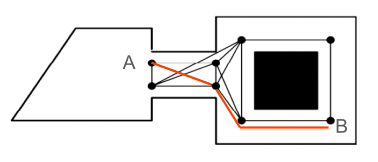
\includegraphics[width=0.6\textwidth]{figures/kap3/games-navigation-waypoints.png}
    \caption{Spielnavigation mit Wegpunkten}
    \label{fig:game-navigation-waypoitns}
\end{figure}

Dieser Ansatz mit Wegpunkten schr�nkt jedoch die Bewegung der Spielfiguren stark ein. Dieser Ansatz mit Wegpunkten schr�nkt jedoch die Bewegung der Spielfiguren stark ein. Ein besserer Ansatz ist die Verwendung von Polygon-Netze.

Bereiche, in denen sich die Figuren frei bewegen k�nnen, werden als Polygone dargestellt, und diese Bereiche sind durch Knoten miteinander verbunden. Bei diesem Ansatz k�nnen sich die Figuren freier bewegen, und der Ansatz kann weiterhin mit bekannten Algorithmen wie A* berechnet werden.

\begin{figure}[H]
    \centering
    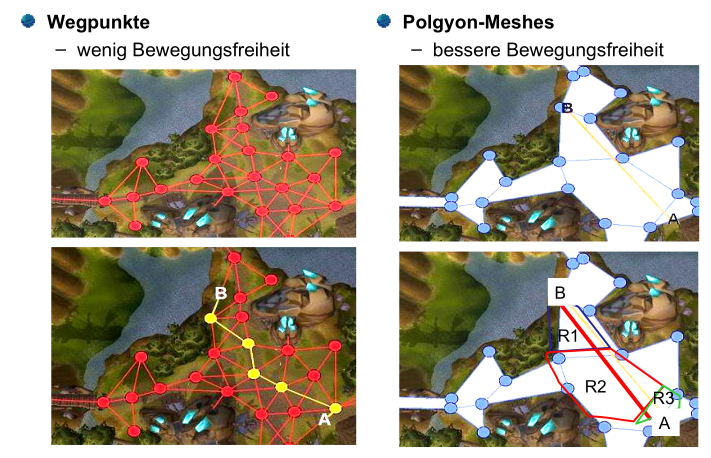
\includegraphics[width=\textwidth]{figures/kap3/waypoints vs polygon.png}
    \caption{Spielnavigation mit Polygon-Meshes vs Wegpunkte}
    \label{fig:game-navigation-navmesh}
\end{figure}